\documentclass[12pt]{article}
\usepackage{coursenote}
\begin{document}
\title{STAT 611 Part 2}
\subtitle{Stationary Processes\\
\normalsize{(chapters 4, 6.1--6.3, 6.5--6.6, 7.1--7.5, 8, 9.1--9.6)}}
\maketitle

\section{General linear processes}

General formula:
\begin{equation}\label{eq:general-linear}
Y_t = e_t + \psi_1 e_{t-1} + \psi_2 e_{t-2} + \dotsb,
\end{equation}
where
$e_t \overset{\text{iid}}{\sim} N(0, \sigma^2)$.
(However, it would have been more consistent with similar models,
in particular MA models, to use
`$-$' in front of the $\psi$'s.)

Reasons for talking about this form:
\begin{enumerate}
\item It's simple because the $e$'s are iid.
    For example, it's trivial to find $E(Y_t)$ and $\var(Y_t)$.
    Covariances are also easy to derive.
\item All the stationary model we're concerned about
    can be written in this form.
\end{enumerate}

Comments:
\begin{enumerate}
\item
$Y_t$ is a linear combination of \emph{current and past} (but not
    future) $e$'s.

\item There may be infinite or finite
    (the $\psi$'s at a certain lag in the past and older are 0) terms.

\item The first coefficient, $\psi_0$, is set to 1 without loss of
    generality.

\item The $e$'s are NOT observed; they are a model device.
   The $Y$'s are the observed values.
   We \emph{assume} the $Y$'s have occurred this way.
   (Recall a similar understanding for linear models.)

\item This form is general; it may or may not be the most convenient for a
    particular purpose. For certain purposes we may want to use
    alternative (but equivalent) forms.

\item This form implies $E(Y_t) = 0$.
   This is OK for much discussion of models because adding a constant to it
   wouldn't affect the correlations.
   When we fit actual data, we may allow a constant mean to be
   estimated.

\item We study stationary processes.
   This needs the $\psi$'s to satisfy certain conditions.
   In particular, the condition is that
   the coefficients $\psi_j$ are \emph{absolutely summable}:
   \[
   \sum_{j=1}^\infty |\psi_j| < \infty.
   \]
   Note that
   if (\ref{eq:general-linear}) has a \emph{finite} number of terms,
   this condition is satisfied with whatever values of the coefficients.
\end{enumerate}

In general, given a particular form of the series, we'll study
\begin{itemize}
\item its ACF (autocorrelation function)  $\rho_k$, $k=1,2\dotsc$;
\item its variance $\gamma_0$;
\item its PACF (partial autocorrelation function)  $\phi_{kk}$, $k=1,2\dotsc$;
\item discuss how the $\rho_k$ and $\phi_{kk}$ behaves,
    in particular,
    their signs (positive? negative? oscillating?),
    whether they gradually die off or abruptly cut off,
    the pace of their decay,
    and how these behaviours are affected by the coefficients of the
    model.
    We always want to look at a plot of $\rho_k$, $\phi_{kk}$
    versus the lag $k$.
\end{itemize}

\section{MA models}

\[
Y_t = e_t - \theta_1 e_{t-1} - \theta_2 e_{t-2}
    - \dotsb - \theta_q e_{t-q}
\]
``order $q$'': MA($q$).
This is just a special form of~(\ref{eq:general-linear}) with finite $q$.

Because MA is a linear combination of \emph{independent} $e$'s,
it's quite easy to work out its variance and auto-covariances.

\subsubsection{Variance}

\[
\gamma_0 = (1 + \theta_1^2 + \theta_2^2 +\dotsb+ \theta_q^2) \sigma^2_e
\]

\subsubsection{ACF}

\[\begin{split}
\gamma_k
&= \cov\bigl(
    e_t - \theta_1 e_{t-1} -\dotsb- \theta_q e_{t-q},\,
    e_{t-k} - \theta_1 e_{t-1-k} -\dotsb- \theta_q e_{t-q-k}
    \bigr)
\\
&= \bigl(
    -\theta_k + \theta_{k+1} \theta_1 + \theta_{k+2} \theta_2
    +\dotsb+ \theta_q \theta_{q-k}
    \bigr)\sigma^2_e
\end{split}
\]
if $k \le q$ (otherwise there's no common $e$, hence $\gamma$ is zero).

\exercise
How to identify the overlapping terms?

Subsequently, the ACF is
\[
\rho_k = \frac{\gamma_k}{\gamma_0} = \dotsb
.
\]
Note $\rho_k$ is a function of $\theta$'s only;
it does not involve $\sigma_e^2$.

\emph{In a MA($q$) process, ACF cuts off after lag $q$.}
Usually, the coefficients
$\theta_j$ decreases in absolute value as $j$ increases,
hence the ACF decreases in absolute value until it disappears.

\alert Verify that \emph{MA processes are always stationarity}.

\example
MA($1$) (dropping subscript 1 from $\theta$):
\[
\gamma_0 = (1 + \theta^2) \sigma^2_e,\quad
\gamma_1 = -\theta \sigma_e^2,\quad
\rho_1 = -\frac{\theta}{1 + \theta^2},\quad
\rho_2 = \rho_3 =\dotsb= 0
\]

\alert
1. The sign of $\rho_1$ is opposite to that of $\theta$.

2. $|\rho_1| \le \frac{1}{2}$ (To prove this, use
$\left|\theta + \frac{1}{\theta}\right| \ge 2$.)

\example
\[
Y_t = e_t - 0.8 e_{t-1}
\]

How can we we simulate this process?

\begin{verbatim}
> theta <- .8
> e <- rnorm(30)
> e1 <- e[-length(e)]
> e2 <- e[-1]
> y <- e1 - theta * e2
> pdf(file = 'lect02-1.pdf', width = 5, height = 4)
> plot(y, type = 'b', xlab = 't', ylab = 'Y')
> dev.off()
X11cairo 
       2 
\end{verbatim}

Note $\rho_1 = \frac{-0.8}{1 + 0.64} = -0.49$.

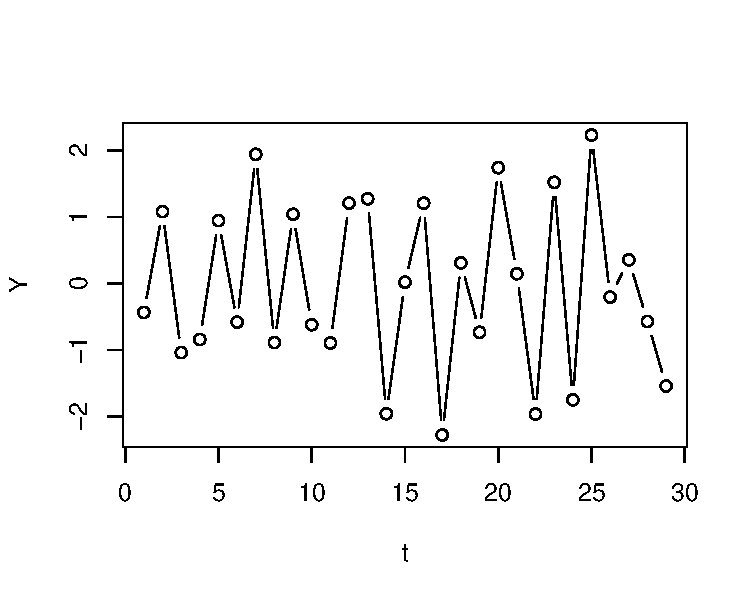
\includegraphics[width=.7\textwidth]{lect02-1.pdf}

Check lag-1 pairs, they should show some negative correlation.

\begin{verbatim}
> pdf(file = 'lect02-2.pdf', width = 5, height = 5)
> plot(y[-length(y)], y[-1], xlab = 'Y[t]', ylab = 'Y[t-1]')
> dev.off()
X11cairo 
       2 
\end{verbatim}

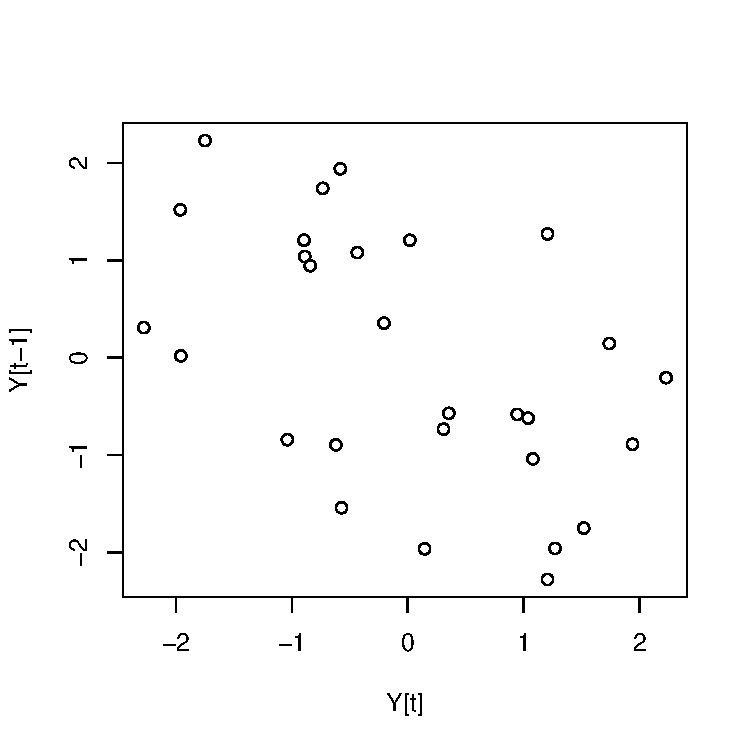
\includegraphics[width=.7\textwidth]{lect02-2.pdf}

We can also check by graph that lag-2 pairs show no correlation.

\example MA($2$), p.~62.

\section{AR models}

\[
Y_t = e_t + \phi_1 Y_{t-1} + \phi_2 Y_{t-2} +\dotsb+ \phi_p Y_{t-p}
\]
Order $p$: AR($p$).
This is the ``current'' random term ($e_t$) plus a linear regression with its
own past---the $p$ most recent past values
(hence the name ``regression'').

Stationarity is assumed (the condition for its stationarity is discussed
shortly).

Under the stationarity assumption,
taking expectation on both sides, we get
\begin{align*}
E(Y_t) &= E(e_t) + \phi_1 E(Y_{t-1}) +\dotsb+ \phi_p E(Y_{t-p})\\
\intertext{or}
\mu &= (\phi_1 +\dotsb + \phi_p) \mu
\end{align*}
hence $\mu \equiv E(Y_t) = 0$ unless
$1 - \phi_1 -\dotsb - \phi_p = 0$.
(We'll see that stationarity requires
$1 - \phi_1 -\dotsb - \phi_p \ne 0$.)


\alert
The notational conventions (at least in this book) for MA and AR models.

\alert
We will use this assumption repeatedly:
$e_t$ is independent of $Y_{t-1}$, $Y_{t-2}$, ..., that is, previous
$Y$'s.
This claim is backed by the assumption (and requirement) that
the $Y_t$ in the AR($p$) can be equivalently expressed as
\[
Y_t = e_t + \psi_1 e_{t-1} + \psi_2 e_{t-2} +\dotsb
,
\]
(note: noise of \emph{past}, not future times)
and the $e_j$'s are independent of each other.
This property is called ``causality'' and will be discussed later.

\alert
However, $e_t$ is not independent of the current $Y_t$,
and we have
\[
E\bigl[e_t Y_t\bigr]
= E\bigl[e_t (e_t + \phi_1 Y_{t-1} +\dotsb+ \phi_p Y_{t-p}\bigr]
= E(e_t^2)
= \sigma_e^2
\]
This is connected to the property of ``causality'' to be introduced
later.


\alert
This section of the note stresses consistent strategies whether the
order is 1, 2, or more. It's cleaner than counterparts of
section~4.3 of the book.

\subsection{AR(1)}

\begin{equation}\label{eq:AR1}
Y_t = e_t + \phi Y_{t-1}
\end{equation}

\subsubsection{ACF}

Multiply both sides of (\ref{eq:AR1}) by $Y_{t-k}$:
\[
Y_t Y_{t-k} = e_t Y_{t-k} + \phi Y_{t-1} Y_{t-k}
\]
Take expectations:
\[
E\bigl[Y_t Y_{t-k}\bigr]
= E[e_t] E[Y_{t-k}] + \phi E\bigl[Y_{t-1} Y_{t-k}\bigr]
\]
(b/c of the independence of $e_t$ and $Y_{t-k}$).
Using the zero-mean assumption, this becomes
\[
\gamma_k = \phi \gamma_{k-1}
\]
Divide by $\gamma_0$:
\[
\rho_k = \phi \rho_{k-1}
\]
This is a recursive relation that needs the previous $\rho$
to calculate the next $\rho$.
Let's take $k=1$ to get an equation for $\rho_1$:
\[
\rho_1 = \phi \rho_0 = \phi
\]
This is called the \emph{Yule-Walker equation}.
For AR(1), this gives $\rho_1$ directly.
All other $\rho$'s follow by recursion:
\begin{align*}
\rho_1 &= \phi\\
\rho_2 &= \phi \rho_1 = \phi^2\\
\rho_3 &= \phi \rho_2 = \phi^3\\
\dotsb &= \dotsb\\
\rho_k &= \phi^k
\end{align*}

(In fact, we don't have to start the recursion with $\rho_1$.
The known $\rho_0 = 1$ already makes the recursion perfectly ready for use.)

\alert
The ACF of AR(1) decays exponentially fast,
but does not reduce to exactly 0.

\subsubsection{Variance}

Multiply both sides of (\ref{eq:AR1}) by $Y_t$:
\[
Y_t Y_t = e_t Y_t + \phi Y_{t-1} Y_t
\]
Take expectations and use the zero-mean assumption:
\[
\gamma_0
= E[e_t Y_t] + \phi \gamma_1
= \sigma_e^2 + \phi \rho_1 \gamma_0
\]
hence
\[
\gamma_0 = \frac{\sigma_e^2}{1 - \phi \rho_1}
\]
The known $\rho_1$ can be substituted to get
$
\gamma_0 = \frac{\sigma_e^2}{1 - \phi^2}
$.

\subsection{AR(2)}

\begin{equation}\label{eq:AR2}
Y_t = e_t + \phi_1 Y_{t-1} + \phi_2 Y_{t-2}
\end{equation}

\subsubsection{ACF}

Multiply both sides of (\ref{eq:AR2}) by $Y_{t-k}$:
\[
Y_t Y_{t-k}
= e_t Y_{t-k} + \phi_1 Y_{t-1} Y_{t-k} + \phi_2 Y_{t-2} Y_{t-k}
\]
Take expectations and divide by $\gamma_0$:
\[
\rho_k = \phi_1 \rho_{k-1} + \phi_2 \rho_{k-2}
\]
This is a recursion that uses two previous $\rho$'s to get the next.
Let's take $k=1,2$ to get an equation system about $\rho_1$ and
$\rho_2$:
\[\begin{split}
\rho_1 &= \phi_1 \rho_0 + \phi_2 \rho_{-1} = \phi_1 + \phi_2 \rho_1
\\
\rho_2 &= \phi_1 \rho_1 + \phi_2 \rho_{0} = \phi_1 \rho_1 + \phi_2
\end{split}
\]
These are called the \emph{Yule-Walker equations}.
Solve to get
\[
\begin{split}
\rho_1 &= \frac{\phi_1}{1 - \phi_2}
\\
\rho_2 &= \frac{\phi_1^2 + \phi_2 - \phi_2^2}{1 - \phi_2}
\end{split}
\]
Then the recursion can proceed to get all $\rho$'s one by one.
This way we get the values numerically,
but not an analytical formula for $\rho_k$ as an explicit function
of the coefficients $\phi$'s.

(In fact, we only need to take $k=1$ to get the solvable equation for
$\rho_1$; then $\rho_0$ and $\rho_1$ will get the recursion rolling.
Check that the $\rho_2$ above follows the recursion.)

Behavior of the ACF (how it decays) will be discussed shortly.

\subsubsection{Variance}

Multiply both sides of (\ref{eq:AR2}) by $Y_t$:
\[
Y_t Y_t = e_t Y_t + \phi_1 Y_{t-1} Y_t + \phi_2 Y_{t-2} Y_t
\]
Take expectations and use the zero-mean assumption:
\[
\gamma_0 = E[e_t Y_t] + \phi_1 \rho_1 \gamma_0 + \phi_2 \rho_2 \gamma_0
\]
hence
\[
\gamma_0
= \frac{\sigma_e^2}{1 - \phi_1 \rho_1 - \phi_2 \rho_2}
\]
The known $\rho_1$ and $\rho_2$ can be plugged in
to get a formula of $\gamma_0$ in terms of
model parameters $\phi_1$, $\phi_2$, and $\sigma^2_e$.

Note the analogy with the $\gamma_0$ of AR(1).

\subsection{AR($p$)}

\begin{equation}\label{eq:ARp}
Y_t = e_t + \phi_1 Y_{t-1} +\dotsb+ \phi_p Y_{t-p}
\end{equation}

\subsubsection{ACF}

Multiply both sides of (\ref{eq:ARp}) by $Y_{t-k}$:
\[
Y_t Y_{t-k}
= e_t Y_{t-k} + \phi_1 Y_{t-1} Y_{t-k} +\dotsb+ \phi_p Y_{t-p} Y_{t-k}
\]
Take expectations and divide by $\gamma_0$:
\[
\rho_k = \phi_1 \rho_{k-1} + \dotsb + \phi_p \rho_{k-p}
\]
This is a recursion that uses $p$ previous $\rho$'s to get the next.
Take $k=1,\dotsc,p$, we get
\[\begin{split}
\rho_1 &= \phi_1 + \phi_2 \rho_1 + \phi_3 \rho_2 +\dotsb+
            \phi_p\rho_{p-1}
\\
\rho_2 &= \phi_1 \rho_1 + \phi_2 + \phi_3 \rho_1 +\dotsb+
            \phi_p\rho_{p-2}
\\
\vdots &
\\
\rho_p &= \phi_1 \rho_{p-1} + \phi_2 \rho_{p-2} +\dotsb+
            \phi_p
\end{split}
\]
These are called the \emph{Yule-Walker equations}.
They are $p$ equations with $p$ unknowns.
Solve to get
$\rho_1,\dotsc,\rho_p$.
Then the recursion can proceed to get all $\rho$'s one by one,
numerically.

(In fact,
it suffices to take $k=1,\dotsc,p-1$ to get $p-1$ equations
for $\rho_1,\dotsc,\rho_{p-1}$.
Solve,
then $\rho_0,\rho_1,\dotsc,\rho_{p-1}$ get the recursion rolling.)

Behavior of the ACF (how it decays) will be discussed shortly.

\subsubsection{Variance}

Multiply both sides of (\ref{eq:ARp}) by $Y_t$:
\[
Y_t Y_t = e_t Y_t + \phi_1 Y_{t-1} Y_t +\dotsb+ \phi_p Y_{t-p} Y_t
\]
Take expectations and use the zero-mean assumption:
\[
\gamma_0 = E[e_t Y_t] + \phi_1 \rho_1 \gamma_0 +\dotsb+ \phi_p \rho_p \gamma_0
\]
hence
\[
\gamma_0
= \frac{\sigma_e^2}{1 - \phi_1 \rho_1 - \dotsb - \phi_p \rho_p}
\]
Noticing $\rho_1$,..., $\rho_p$ are now known
(numerically),
plug in to get the value of $\gamma_0$.


\subsection{Simulation}

\begin{verbatim}
> simul.ar <- function(n, phi, sigma = 1)
+ {
+     p <- length(phi)
+ 
+     et <- rnorm(n) * sigma
+     y <- numeric(n)
+     for (i in 2 : n)
+     {
+         k <- min(p, i-1)
+         y[i] <- et[i] + sum(y[(i-1) : (i-k)] * phi[1:k])
+     }
+     y
+ }
\end{verbatim}

\begin{verbatim}
> y <- simul.ar(500, .8)
> pdf(file = 'lect02-3a.pdf', width = 8, height = 3)
> plot(y, type = 'l', xlab = 'Time', ylab = 'Y', cex = .5)
> dev.off()
X11cairo 
       2 
> pdf(file = 'lect02-3b.pdf', width = 8, height = 3)
> acf(y, main = NA)
> dev.off()
X11cairo 
       2 
> 
> y <- simul.ar(500, -.5)
> pdf(file = 'lect02-4a.pdf', width = 8, height = 3)
> plot(y, type = 'l', xlab = 'Time', ylab = 'Y', cex = .5)
> dev.off()
X11cairo 
       2 
> pdf(file = 'lect02-4b.pdf', width = 8, height = 3)
> acf(y, main = NA)
> dev.off()
X11cairo 
       2 
> 
> y <- simul.ar(500, c(.1, .5))
> pdf(file = 'lect02-5a.pdf', width = 8, height = 3)
> plot(y, type = 'l', xlab = 'Time', ylab = 'Y', cex = .5)
> dev.off()
X11cairo 
       2 
> pdf(file = 'lect02-5b.pdf', width = 8, height = 3)
> acf(y, main = NA)
> dev.off()
X11cairo 
       2 
> 
> y <- simul.ar(500, c(.8, -.5))
> pdf(file = 'lect02-6a.pdf', width = 8, height = 3)
> plot(y, type = 'l', xlab = 'Time', ylab = 'Y', cex = .5)
> dev.off()
X11cairo 
       2 
> pdf(file = 'lect02-6b.pdf', width = 8, height = 3)
> acf(y, main = NA)
> dev.off()
X11cairo 
       2 
> 
\end{verbatim}

\begin{center}
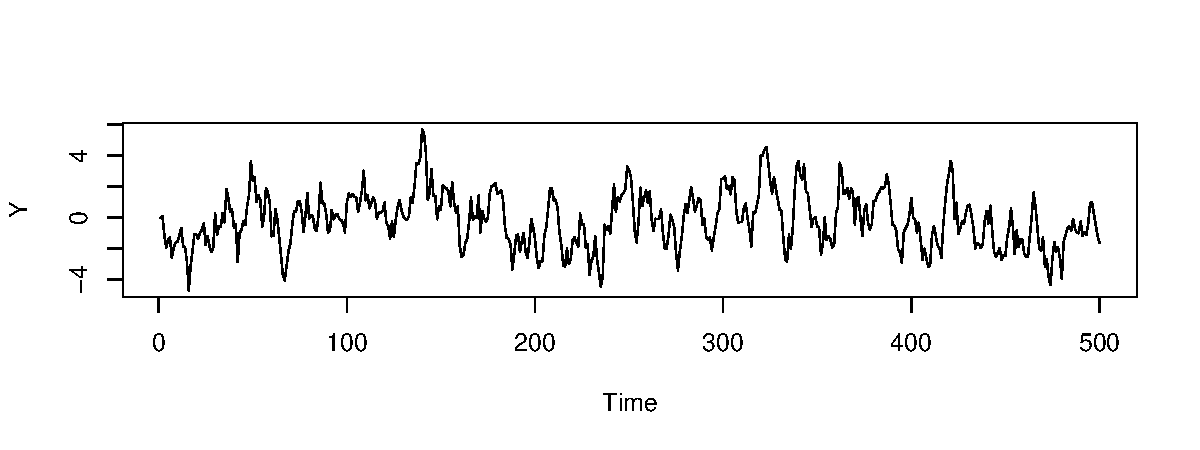
\includegraphics[width=1.2\textwidth]{lect02-3a.pdf}
\vspace*{-20mm}

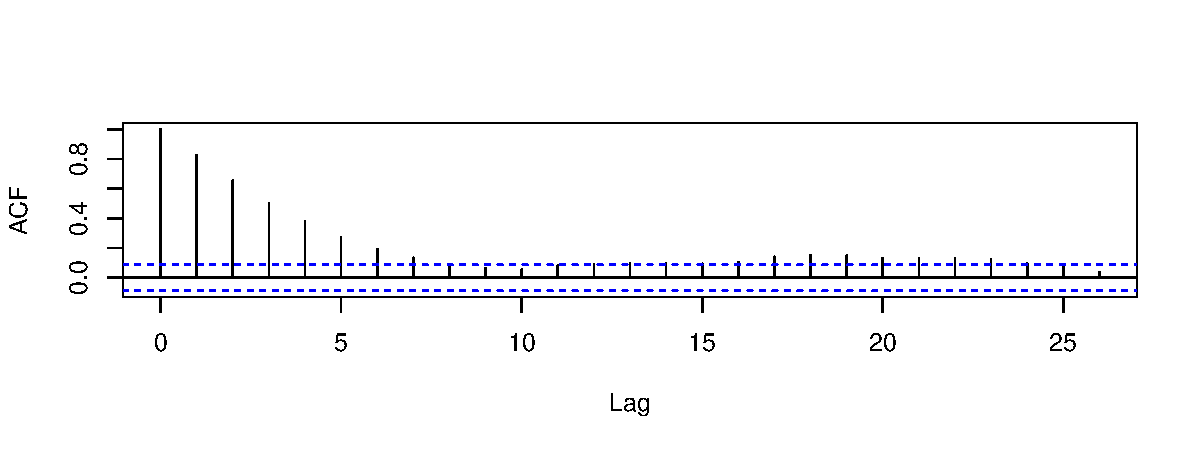
\includegraphics[width=1.2\textwidth]{lect02-3b.pdf}
\end{center}

\begin{center}
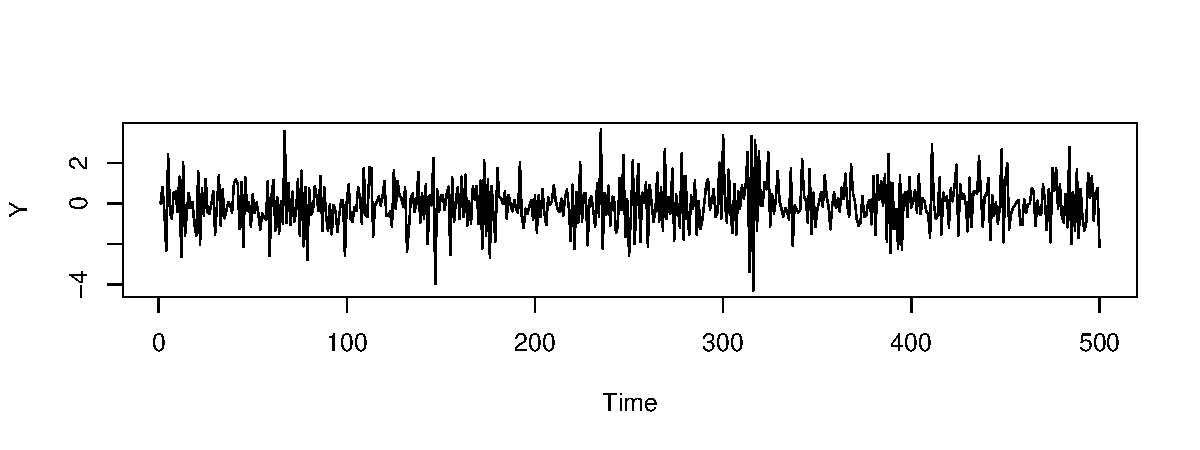
\includegraphics[width=1.2\textwidth]{lect02-4a.pdf}
\vspace*{-20mm}

\includegraphics[width=1.2\textwidth]{lect02-4b.pdf}
\end{center}

\begin{center}
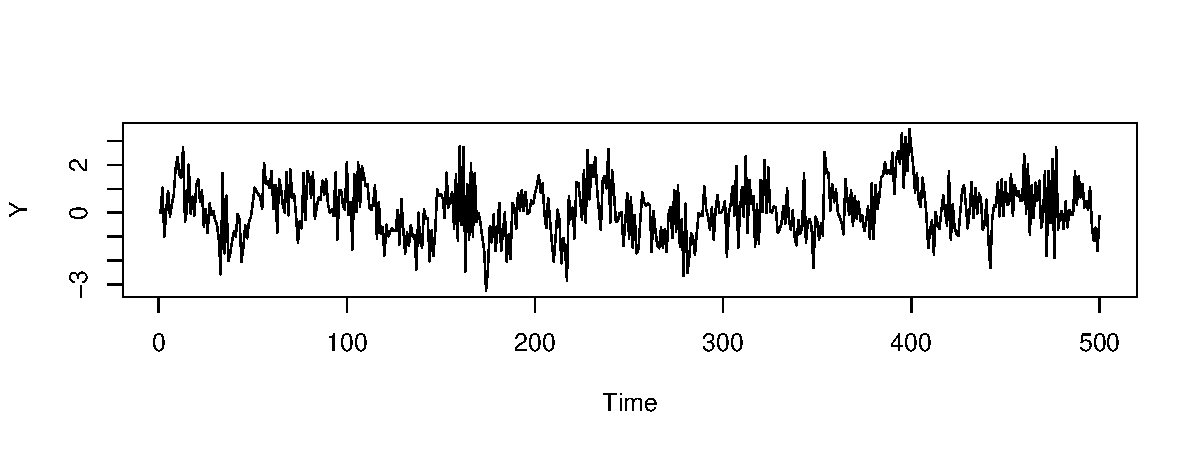
\includegraphics[width=1.2\textwidth]{lect02-5a.pdf}
\vspace*{-20mm}

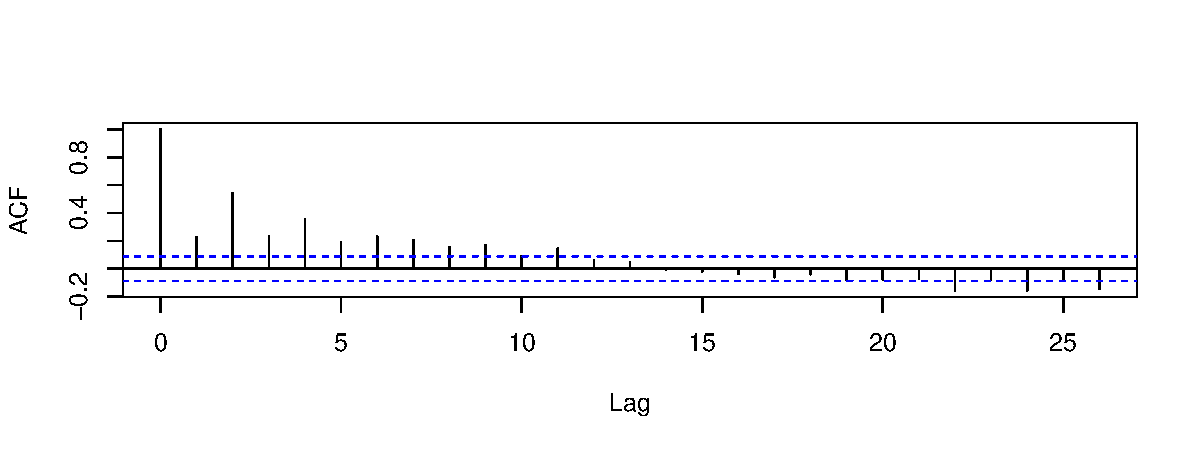
\includegraphics[width=1.2\textwidth]{lect02-5b.pdf}
\end{center}

\begin{center}
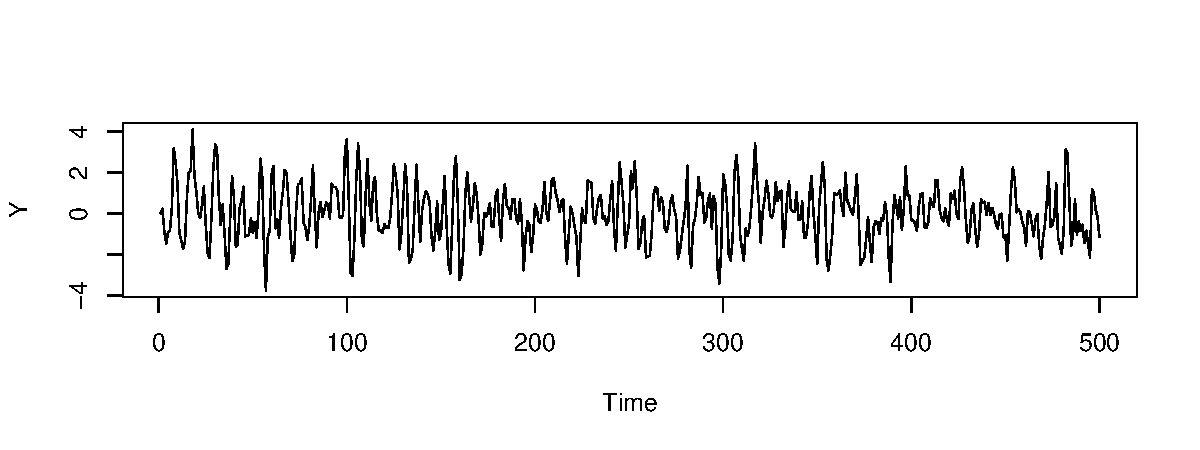
\includegraphics[width=1.2\textwidth]{lect02-6a.pdf}
\vspace*{-20mm}

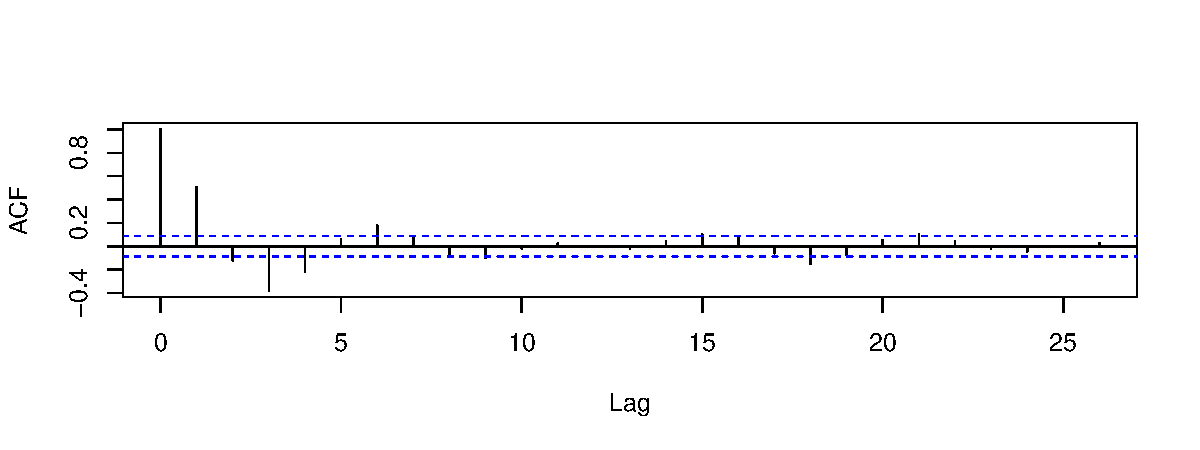
\includegraphics[width=1.2\textwidth]{lect02-6b.pdf}
\end{center}

\exercise
Play with different values of $\phi$'s
(including some that make the process non-stationary).

\section{Backshift operator}

(Page 106.)

We use the symbol $B$. (In some books it's called ``lag operator'' and
denoted by $L$.)

By definition, let
$B Y_t$ mean $Y_{t-1}$.

Then,
$B^2 Y_t = B B Y_t = B Y_{t-1} = Y_{t-2}$.

In general,
$B^s Y_t = Y_{t-s}$.

In particular, $B^0 Y_t = Y_t$.

Differencing:
\[
\nabla Y_t = Y_t - Y_{t-1} = (1 - B) Y_t
\]
\[
\nabla^d Y_t = (1 - B)^d Y_t
\]

AR($p$),
$
Y_t = e_t + \phi_1 Y_{t-1} + \dotsb + \phi_p Y_{t-p}
$,
can be written as
\[
Y_t = e_t + (\phi_1B + \phi_2B^2 + \dotsb + \phi_pB^p) Y_t
\]
or better,
\[
(1 - \phi_1B - \phi_2B^2 - \dotsb - \phi_pB^p) Y_t = e_t
\]

\definition
\textbf{Autoregressive operator}
\[
\phi(B) = 1 - \phi_1 B - \phi_2 B^2 - \dotsb - \phi_p B^p
\]
\definition
\textbf{Moving average operator}
\[
\theta(B) = 1 - \theta_1 B - \theta_2 B^2 - \dotsb - \theta_q B^q
\]
Write the AR($p$) model as
\[
\phi(B) Y_t = e_t
\]
and the MA($q$) model as
\[
Y_t = \theta(B) e_t
\]
To make the notation self-sufficient with order information, we could
write
$\phi_p(B) Y_t = e_t$ and $Y_t = \theta_q(B) e_t$,
such as
$\phi_3(B) Y_t = e_t$ and $Y_t = \theta_2(B) e_t$.

\alert
Now we see whey we use ``+'' in front of $\phi_i$ but
``-'' in front of $\theta_j$.
However, some books use ``+'' in both cases.

\definition
AR($p$) \emph{characteristic polynomial}:
\[
\phi(x) = 1 - \phi_1 x - \phi_2 x^2 -\dotsb- \phi_p x^p
\]
AR($p$) \emph{characteristic equation}:
\[
\phi(x) = 0
\]
(These could also be written as
$\phi(z)$ or even $\phi(B)$.
$x$ or $z$ or $B$ is just a place holder;
it doesn't matter what to use here.
The real thing is the coefficients.)

Properties of the roots of the characteristic equation
are very important in discussion of properties of the AR($p$) process.
(Note that it's also common to speak of the ``roots'' of a polynomial,
which refer to roots of the equation.)

Similarly define characteristic polynomial and characteristic equation
of a MA($q$) model.

\definition
MA($q$) \emph{characteristic polynomial}:
\[
\theta(x) = 1 - \theta_1 x - \theta_2 x^2 -\dotsb- \theta_q x^p
\]
MA($q$) \emph{characteristic equation}:
\[
\theta(x) = 0
\]


\section{Explosive AR models and causality}

Consider $Y_t = e_t + \phi Y_{t-1}$.

We know $Y_t$ is nonstationary if $\phi = 1$ (random walk).

If $|\phi| < 1$, we have
\[
Y_t
= e_t + \phi(e_{t-1} + \phi Y_{t-2})
= \dotsb
= e_t + \phi e_{t-1} + \phi^2 e_{t-2} + \phi^3 e_{t-3} +\dotsb
= \sum_{j=0}^{\infty} \phi^j e_{t-j}
\]
Because $|\phi| < 1$, the magnitude of $\phi^j$ quickly decreases,
and so the above series converges,
hence it's a meaningful representation.

If $|\phi| > 1$,
the series $\phi^j$ does not converge
hence $Y_t = \sum_{j=0}^\infty \phi^j e_{t-j}$ is not usable.
It's called an ``explosive'' AR model.

However, if we define
$\epsilon_t = -e_t /\phi$, and write
$Y_{t-1} = \epsilon_t + \frac{1}{\phi} Y_t$, or better,
\[
Y_t = \epsilon_{t+1} + \frac{1}{\phi} Y_{t+1}
,
\]
then since $\bigl|\frac{1}{\phi}\bigr| < 1$,
we have
\[
Y_t = \sum_{j=0}^{\infty} (1/\phi)^{j} Y_{t+j}.
\]
Now the coefficients converges,
hence it's a meaningful series.
This shows that
\emph{if it's mathematically equivalent for time
to go backward and forward},
then
$|\phi| > 1$ and $|\phi| < 1$
are equivalent \emph{after some transformation}.

\emph{In practice}, however, it's not very useful to
express $Y_t$ in terms of \emph{the future}.
Moreover,
the $|\phi| > 1$ case has to be somehow transformed to be nice.
So we do not like this case.

\definition
\textbf{Causality}\\
The process $\{Y_t\}$ represented by the AR($p$) model
is \emph{causal},
or is a \emph{causal function of $\{e_t\}$},
if there exist constants $\{\psi_j\}$ such that
$\sum_{j=0}^\infty |\psi_j| < \infty$ and
\[
Y_t = \sum_{j=0}^\infty \psi_j e_{t-j}
\quad
\text{for all $t$.}
\]
In other words,
causality means $Y_t$ can be expressed by \emph{current and past} $e$.
In still other words,
a ``causal'' AR process is one that can be expressed as
a MA process.
(This MA process is invariably an infinite series.)

(It seems ``causal'' and ``stationary'' AR are interchangeable terms,
but I have not seen sources to confirm this.)


\theorem
\textbf{Condition for causality}\\
Causality is equivalent to the condition
\[
\phi(x) = 1 - \phi_1x - \phi_2x^2 - \dotsb \phi_p x^p \ne 0
\quad
\text{for all $|x| \le 1$.}
\]
In other words,
all roots of $\phi(x) = 0$ are \emph{outside} the unit circle.


\textbf{Special cases:}

For AR(1), a necessary and sufficient condition is $|\phi| < 1$.

For AR(2), a necessary and sufficient condition is~(4.3.11), p.~72. Also
see Exhibit~4.17, p.~72.

For AR($p$) in general, a necessary but not (necessarily) sufficient
condition is~(4.3.28), p.~76.

When we simulate AR processes, the $\phi$'s should be chosen
with attention to these conditions.


\section{Non-uniqueness of MA models and invertibility}

Consider $Y_t = e_t - \theta e_{t-1}$.

We have seen that
$\gamma_0 = (1 + \theta^2) \sigma^2_e$,
$\rho_1 = -\frac{\theta}{1 + \theta^2}$,
$\rho_2 = \rho_3 = \dotsb = 0$.

Define model
$Y_t = \theta e_t - \frac{1}{\theta} e_{t-1}$.
We can see this model has the same
$\gamma_0$ (note the change of the error variance)
and $\rho$'s as the first one.
And both models have $E(Y_t) = 0$.

Therefore as far as modeling $Y_t$ is concerned,
these two are the \emph{same model}.
(Their noise levels are different but those are not observed;
they are an auxiliary device for modeling $Y_t$.)

Then, which one to choose?

For an AR model,
we want a \emph{causal} one, that is,
$Y_t$ can be expressed by \emph{current and past} $e$'s.
Analogously,
for a MA model,
we want one in which
$e_t$ can be expressed by \emph{current and past} $Y$'s.
A reason for this desire is that we want to work with $e$'s;
and only when $e_t$ can be expressed by current and past $Y$'s can
we calculate the $e$'s up to the current time.
Such a MA model is called \emph{invertible}.

\definition
\textbf{Invertibility}\\
The process $\{Y_t\}$ represented by
the MA($q$) model is \emph{invertible}
if there exist constants $\{\pi_j\}$ such that
$\sum_{j=0}^\infty |\pi_j| < \infty$ and
\[
e_t = \sum_{j=0}^\infty \pi_j Y_{t-j}
\quad
\text{for all $t$.}
\]
In other words,
invertibility means $e_t$ can be expressed by \emph{current and past} $Y$.
In still other words,
an ``invertible'' MA process is one that can be expressed as an AR process.
(This AR process is invariably an infinite series.)

Re-arrange the MA(1) model as
\[
e_t = Y_t + \theta e_{t-1}.
\]
Compare with the AR(1) model
\[
Y_t = e_t + \phi Y_{t-1}
\]
By symmetry, we see
the condition for $\phi$ to make the AR(1) causal
must be the same
condition for $\theta$ to make the MA(1) invertible.

\theorem
\textbf{Condition for invertibility}\\
Invertibility is equivalent to the condition
\[
\phi(x) = 1 - \theta_1x - \theta_2x^2 - \dotsb \theta_p x^p \ne 0
\quad
\text{for all $|x| \le 1$.}
\]
In other words,
all solutions of $\theta(x) = 0$ have modulus greater than 1.


\section{Properties of ACF of an AR process}

The most important observation about ACF of a MA($q$)
process is that it cuts off after lag $q$.
ACF usually (or probably always) drops quickly before it becomes zero;
but the specific formulae for its nonzero values are less important.

In this section we focus on the behavior of the ACF of an AR($p$)
process.
This ACF does not cut off---it remains nonzero for whatever lag.
But we'll show its magnitude drops rather quickly as the lag increases.

Discussion of the behavior of $\rho_k$ is under the causality assumption
(which stipulates permissible values of the $\phi$'s).

Some discussion can be made based on the formulas for
AR(1) and AR(2) we have derived.

For AR(1), we know $-1 < \phi < 1$ and $\phi_k = \phi^k$.
So,\\
if $\phi > 0$,...\\
if $\phi < 0$,...

For AR(2), the magnitude of $\rho_k$ dies out exponentially fast as $k$
increases. In the case of complex roots of the characteristic equation,
$\rho_k$ displays a damped sine wave behavior. (p.~73)

These statements about the behavior of $\rho$ in AR is general:
they die out exponentially fast,
either with the same sign or in a sinusoidal fashion.

In general,
suppose
\[
\phi(x) = \prod_{i=1}^p (1 - g_i x)
\]
that is,
the roots of the characteristic equation are
$g_1^{-1},\dotsc,g_p^{-1}$.
The general solution of the autocorrelations are
\[
\rho_k = a_1 g_1^k + a_2 g_2^k + \dotsc + a_p g_p^k.
\]
For causality we require $|g_i| < 1$.
Thus two situations can arise if we assume the roots are distinct.
\begin{enumerate}
\item A root $g_i^{-1}$ is real, in which case the term
    $a_i g_i^k$ decays to zero geometrically as $k$ increases.
    This is called a ``damped exponential''.
\item A pair of roots, $g_i^{-1}$ and $g_j^{-1}$, are complex
conjugates, in which case they contribute the following term,
\[
a_i g_i^k + a_j g_j^k
= d^k \sin (2\pi f k + F)
,
\]
to $\rho_k$.
This is a damped sine wave, with damping factor $d$.
\end{enumerate}
In general,
the autocorrelation function of a causal AR process will consist of a
mixture of damped exponentials and damped sine waves.


\section{ARMA models}

General form of ARMA($p,q$): (4.4.1), p.~77.
\[
Y_t = \phi_1 Y_{t-1} + \dotsb + \phi_p Y_{t-p}
    + e_{t} - \theta_1 e_{t-1} - \dotsb - \theta_q e_{t-q}
\]
This is written concisely as
\[
\phi(B) Y_t = \theta(B) e_t
\]


Appendix~C, p.~85, describes a procedure
for finding the $\gamma_0$, $\rho_1,...$ for ARMA($p,q$):
\begin{enumerate}
\item Find the coefs $\psi_0,\psi_1,\dotsc$ for the ``general linear
process'' representation of $Y_t$; see (4.C.1), p.~85, and (4.4.7),
p.~79. (The book uses `$+$' in front of the $\psi$'s;
but it's better to use `$-$' to be consistent with the treatment of
$\theta$'s.)
\item Note $Y_t$ is correlated with past $e$'s but uncorrelated with
future $e$'s.
Using the $\psi$ form, it's easy to find
$E(Y_t e_{t-k})$, $k\ge 0$, because $Y_t$ is expressed as a linear
function of iid $e$'s.
\item Multiply $Y_{t-k}$ on both sides of the ARMA form of $Y_t$, then
take expectation.
The AR terms give $\gamma$'s.
The MA terms are obtained using the $\psi$'s as described above.
\item Take $k$ to be $0,1,\dotsc,p$,
to get a system of $p$ equations
for $\gamma_0, \gamma_1,\dotsc, \gamma_p$.
Solve the system to get
$\gamma_0,\dotsc, \gamma_p$, hence $\rho_1,\dotsc,\rho_p$.
\item If $q > p$, use the same procedure to get
$\gamma_{p+1},\dotsc,\gamma_{q}$ one at a time.
This will use the previously obtained $\gamma_0,\dotsc,\gamma_p$.
One equation (not a system equations) at a time, but not a simple
recursion.
\item For $k>\max(p,q)$, multiply $Y_{t-k}$ on both sides of the ARMA form of
$Y_t$, take expectation. The $e$ terms all vanish (because they are all
in the future of $Y_{t-k}$. We get a recursive formula for $\gamma$ or
$\rho$.
\end{enumerate}


% \theorem
% \textbf{Existence and uniqueness}\\
% A stationary solution $\{Y_t\}$ of ARMA($p$, $q$)
% exists (and is also the unique stationary solution) if and only if
% \[
% \phi(x) = 1 - \phi_1x - \phi_2x^2 - \dotsb \phi_p x^p \ne 0
% \quad
% \text{for all $|x| = 1$.}
% \]
% In other words,
% no root of $\phi(x) = 0$ sits on the unit circle.
% 
% \alert
% A stationary solution of
% ARMA(0, $q$) always exists.
% In other words,
% MA models are stationary.

\emph{Causality}:
if $p > 0$, we talk about whether the ARMA process is ``causal''.
The definition is the same as that for an AR process---only
the AR part of the ARMA has an impact on its causality.

\emph{Invertibility}:
if $q > 0$, we talk about whether the ARMA process is ``invertible''.
The definition is the same as that for a  MA process---only
the MA part of the ARMA has an impact on its invertibility.

Similarly,
the conditions for causality and invertibility
are the same for causal AR and invertible MA,
respectively.

In summary,
\begin{enumerate}
\item
Note the MA and AR formulations are the same except the roles
of $Y$ and $e$ are switched. This explain the analogy
between the concepts of causality and invertibility, and their
conditions on the respective coefficients $\phi$'s and $\theta$'s.
\item
When we check causality of ARMA, we check the AR coefficients only
(because the MA part is already ``causal'').
Similarly, when we check invertibility we check the MA coefficients
only.
\item
Similar analogies/contrasts of the AR and MA models exist
for ACF, PACF, and other properties.
\end{enumerate}


\emph{Requirements on ARMA}

``Stationarity'' is explicitly required in the definition
of ARMA.
In addition we require it to be
\begin{enumerate}
\item causal;
\item invertible;
\item in the simplest (lowest-order) form.
\end{enumerate}

The third requirement means there should be no common factors in
$\phi(B)$ and $\theta(B)$.
We'll have an example
(Example~3.5, page~93, and
Example~3.6, page~96, Shumway and Stoffer).
But this requires knowledge about polynomials which is beyond this
course.


\section{Conversion between various forms}

\subsection{MA form, or $\psi$ form}

Page 55, (4.1.1):
\begin{equation}\label{eq:psi-form}
Y_t = e_t - \psi_1 e_{t-1} - \psi_2 e_{t-2} -\dotsb
\end{equation}
or
$
Y_t = \psi(B) e_t
$.

Page 57, (4.2.1):
\begin{equation}\label{eq:MA-form}
Y_t = e_t - \theta_1 e_{t-1} - \theta_2 e_{t-2}
    -\dotsb - \theta_q e_{t-q}
\end{equation}
or
$
Y_t = \theta(B) e_t
$.

\subsection{AR form, or $\pi$ form}

Page 80, (4.5.5):
\begin{equation}\label{eq:pi-form}
Y_t = e_t + \pi_1 Y_{t-1} + \pi_2 Y_{t-2} +\dotsb
\end{equation}
or
$
\pi(B) Y_{t} = e_t
$.

Page 66, (4.3.1):
\begin{equation}\label{eq:AR-form}
Y_t = e_t + \phi_1 Y_{t-1} + \phi_2 Y_{t-2}
    +\dotsb + \phi_p Y_{t-p}
\end{equation}
or
$
\phi(B) Y_t = e_t
$.

\subsection{ARMA form}

Page 77, (4.4.1):
\begin{multline}\label{eq:ARMA-form}
Y_t = e_t
    + \phi_1 Y_{t-1} + \phi_2 Y_{t-2} +\dotsb+ \phi_p Y_{t-p}
    \\
    - \theta_1 e_{t-1} - \theta_2 e_{t-2} -\dotsb- \theta_q e_{t-q}
\end{multline}
or
$
\phi(B)Y_t = \theta(B) e_t
$.

\subsection{From AR form to MA form}

(Incomplete discussion on page 75.)

Substitute the $\psi$ from (\ref{eq:psi-form})
into the AR form (\ref{eq:AR-form}):
\[
\begin{split}
& e_t - \psi_1 e_{t-1} - \psi_2 e_{t-2} - \psi_3 e_{t-3} -\dotsb
\\
&= e_t
\\
&\phantom{\mathrel{=}\;}
    +
    \phi_1\bigl(e_{t-1} - \psi_1 e_{t-2} - \psi_2 e_{t-3}
        -\dotsb\bigr)
\\
&\phantom{\mathrel{=}\;}
    +
    \phi_2\bigl(e_{t-2} - \psi_1 e_{t-3} - \psi_2 e_{t-4}
        -\dotsb\bigr)
\\
&\phantom{\mathrel{=}\;}
    +\dotsb
\\
&\phantom{\mathrel{=}\;}
    +
    \phi_p\bigl(e_{t-p} - \psi_1 e_{t-p-1} - \psi_2 e_{t-p-2}
        -\dotsb\bigr)
\end{split}
\]
Equate coefficients of the same $e$ on both sides to get
the recursion
\[
\begin{split}
\psi_1 &= -\phi_1 \\
\psi_2 &= \phi_1\psi_1 - \phi_2 \\
\psi_3 &= \phi_1\psi_2 + \phi_2\psi_1 - \phi_3\\
\dotsb &= \dotsb \\
\psi_p &= \phi_1\psi_{p-1} + \phi_2\psi_{p-2}
            +\dotsb + \phi_{p-1} \psi_1 - \phi_p \\
\psi_{p+1} &= \phi_1\psi_{p} + \phi_2\psi_{p-1}
            +\dotsb + \phi_{p-1} \psi_2 + \phi_p\psi_1 \\
\psi_{p+2} &= \phi_1\psi_{p+1} + \phi_2\psi_{p}
            +\dotsb + \phi_{p-1} \psi_3 + \phi_p\psi_2 \\
\dotsb &= \dotsb
\end{split}
\]


Alternatively,
from $\phi(B) Y_t = e_t$ we get
\[
Y_t = \frac{1}{\phi(B)} e_t
\]
But exactly what is
$\frac{1}{\phi(B)}$?
In general,
\[
\frac{1}{\phi(B)}
= 1 - \psi_1 B - \psi_2 B^2 - \dotsb
\]
that is,
\[
(1 - \psi_1 B - \psi_2 B^2 - \dotsb)
    (1 - \phi_1 B - \phi_2 B^2 - \dotsb)
= 1
\]
Expand the multiplication,
work on the coefficients,
and a recursive formulation will emerge.


\subsection{From MA form to AR form}

(Incomplete discussion on page 208.)

Substitute the $\pi$ form (\ref{eq:pi-form})
into the MA form (\ref{eq:MA-form}):
\[\begin{split}
& e_t + \pi_1 Y_{t-1} + \pi_2 Y_{t-2} +\dotsb\\
&= e_t\\
&\phantom{\mathrel{=}\;}
    -\theta_1\bigl(Y_{t-1} - \pi_1Y_{t-2} - \pi_2Y_{t-3}
        -\dotsb\bigr)\\
&\phantom{\mathrel{=}\;}
    -\theta_2\bigl(Y_{t-2} - \pi_1Y_{t-3} - \pi_2Y_{t-4}
        -\dotsb\bigr)\\
&\phantom{\mathrel{=}\;}
    -\dotsb\\
&\phantom{\mathrel{=}\;}
    -\theta_q\bigl(Y_{t-q} - \pi_1Y_{t-q-1} - \pi_2Y_{t-q-2}
        -\dotsb\bigr)
\end{split}
\]
Equate coefficients of the same $Y$ on both sides to get
the recursion
\[\begin{split}
\pi_1 &= -\theta_1\\
\pi_2 &= -\theta_2 + \theta_1\pi_1\\
\pi_3 &= -\theta_3 + \theta_2\pi_1 + \theta_1\pi_2\\
\dotsb &= \dotsb\\
\pi_q &= -\theta_q + \theta_{q-1}\pi_1 + \dotsb + \theta_1\pi_{q-1}\\
\pi_{q+1} &= \theta_q\pi_1 + \theta_{q-1}\pi_2 + \dotsb + \theta_1\pi_{q}\\
\pi_{q+2} &= \theta_q\pi_2 + \theta_{q-1}\pi_3 + \dotsb +
    \theta_1\pi_{q+1}\\
\dotsb &= \dotsb
\end{split}
\]


Alternatively,
from
$Y_t = \theta(B) e_t$
we get
\[
\frac{1}{\theta(B)} Y_t = e_t
\]

Indeed, as we have seen much duality between AR and MA models,
techniques for AR and for MA are the same.


\subsection{From ARMA form to AR and MA forms}

(Incomplete discussion on pages 79 and 208.)

In this general situation the elegance of the $B$ notation
shows most vividly.

Suppose the model is $\phi(B) Y_t = \theta(B) e_t$.

Suppose an alternative form of it is
$\pi(B)Y_t = e_t$
(the existence of which is guaranteed by invertibility), then substitute
this for $e_t$ in ARMA, we get
\[
\phi(B) Y_t = \theta(B) \pi(B) Y_t
\]
that is,
\[
\phi(B) = \theta(B) \pi(B)
\]
Multiply out $\theta(B) \pi(B)$,
equate coefficients of corresponding $B$ polynomials,
we get recursive relations for $\pi$'s.

Suppose an alternative form of it is
$Y_t = \psi(B) e_t$
(the existence of which is guaranteed by causality), then substitute
this for $Y_t$ in ARMA, we get
\[
\phi(B) \psi(B) e_t = \theta(B) e_t
\]
that is,
\[
\phi(B) \psi(B) = \theta(B)
\]
Multiply out $\phi(B) \psi(B)$,
equate coefficients of corresponding $B$ polynomials,
we get recursive relations for $\psi$'s.

We can also write,
directly from $\phi(B)Y_t = \theta(B) e_t$,
\[
Y_t = \frac{\theta(B)}{\phi(B)} e_t
\]
hence $\psi(B) = \theta(B) / \phi(B)$,
and
\[
\frac{\phi(B)}{\theta(B)}Y_t = e_t
\]
hence $\pi(B) = \phi(B) / \theta(B)$.
This is handy for discussion.
But if we want to calculate the actual values of $\psi$'s and $\pi$'s,
writing out the recursive equations might still be the ultimate way to go.


\section{PACF}

\subsection{Definition and properties}

\definition%
(6.2.1), 6.2.2)

When assuming normal noise, these two definitions are equivalent.

\alert[Notation]%
$\phi_{kk}$

\alert[convention]%
$\phi_{00} = 1$
(The book states
$\phi_{11} = 1$ by convention.
This appears to be an error.
Instead, $\phi_{11} = \rho_1$.)

An operational definition is given as follows
(see (6.2.8), p~114).

\definition%
PACF $\phi_{kk}$, $k=0,1,\dotsc$.\\
Define
$\phi_{00} = 0$ and let
$\phi_{kk}$ be the last element of
$\Gamma_k^{-1} \vec{p}_k$,
where
$\Gamma_k = \bigl[\rho(i-j)\bigr]_{i,j=1}^k$
and
$\vec{p}_k = [\rho(1),\rho(2),\dotsc,\rho(k)]'$.


\example
$\phi_{22}$ for a general stationary process: (6.2.3)

\example
Applying (6.2.3) for the special case of AR(1), we get
$\phi_{22} = 0$.

\example
AR($p$) at $k > p$. (6.2.4).

\alert
This result shows that $\phi_{kk} = 0$ for AR($p$)
when $k > p$.
In addition we can show (last paragraph, page~114)
that $\phi_{pp} = \phi_p \ne 0$ for AR($p$).
Both results combined, we see
PACF cuts off right after lag $p$ for AR($p$),
hence the cutting off of (sample) PACF is an indicator
for the order of an AR process.

\alert
PACF for AR behaves much like ACF for MA.
ACF for AR behaves much like PACF for MA.

\example Applying (6.2.3) to MA(1). See (6.2.6).

\alert
PACF for AR($p$) cuts off after lag $p$,
because the auto-regression representation extends only to the past $p$
times.
PACF for MA($q$) does not cut off,
because the AR representation for a MA process
goes back to infinite history.
Similarly,
because an invertible ARMA($p$,$q$) model (with $q > 0$) has an infinite
AR representation, its PCAF will not cut off.

\alert
For ARMA($p$,$q$) with $p>0$ and $q>0$,
neither ACF nor PACF cuts off.
Hence there is no very nice, clear-cut indicators
for the orders $p$ and $q$.

\textbf{Table 6.3}, page~116.


\subsection{Computation}

For a general stationary process,
we can find $\phi_{kk}$ by solving
the Yule-Walker equations~(6.2.8),
which uses $\rho$'s.

\alert
To get $\phi_{kk}$,
we'll need to solve $k$ equations and discard
$k-1$ solutions.

\textbf{A recursive algorithm}: Levinson-Durbin, page 115.


\section{Specification of ARMA models}

Prior to estimating the model parameters,
we need to ``specify'' the model,
meaning here coming up with a reasonable choice (determination)
for the orders $p$ and $q$, based on explorations of the data.
There are a few semi-formal tools to guide this decision.
After the specification, the model parameters
(coefficients and noise variance) will be estimated.
The estimated model will be examined (by ``diagnostics'') to see whether
it seems to be adequate; if not, how to change and specification (and
then re-estimate).

Specification is largely based on the observed (i.e.\@ ``sample'' or
``empirical'') correlation structure, that is, ACF and PACF.
Because we know the theoretical correlation structure of specific
models, the observed structure tells us what the model should be.


Because ACF of MA($q$) cuts off after lag $q$
and PACF of AR($p$) cuts off after lag $p$,
a cut-off ACF indicates a MA model (along with its order)
whereas a cut-off PACF indicates an AR model (along with its order).

In order to judge whether the ACF or PACF has ``cut off'',
that is, reduced to zero, we need to know their \emph{sampling
distributions}, which give us thresholds to be used in tests of of
significance.

If neither ACF nor PACF cuts off,
it's an ARMA model.
To deal with ARMA we learn a new tool called EACF.


\subsection{Computation of sample ACF}

Recall the definition of ACF, (3.6.2), page~46, or (6.1.1), page~109.

\subsection{Sampling distribution of ACF}

ACF is a basic graphical tool for us.
To use it, for example judging whether it has dropped to 0 after certain
lag, we need its sampling distribution and properties.

\theorem
As $n\to \infty$,
\[
r_k \to N(\rho_k, c_{kk}/n)
\]
where $c_{kk}$ is given in (6.1.2).

We won't deal with (6.1.2) or $c_{kk}$ in the general case.
We'll consider the following special cases.

\subsubsection{White noise}

(6.1.3), p.~110

\begin{align*}
\rho_k &= 0,                    \qquad k=1,2,\dotsc\\
\var(r_k) &\approx \frac{1}{n}, \qquad k=1,2,\dotsc\\
\corr(r_i, r_j) &\approx 0,     \qquad i \ne j
\end{align*}

\emph{Usage}

Properties of white noise are used mainly to check whether
the residuals, after fitting some ARMA model,
are white noise.
\begin{enumerate}
\item Check whether $r_k$, $k=1,2,\dotsc$, is within
    $\pm \frac{2}{\sqrt{n}}$.
\item If the first check passes, check whether there are correlations
    among the residuals by looking at the sample ACF or PACF
    \emph{of the residuals}.
\end{enumerate}

If the residuals successfully pass these checks,
meaning it's reasonable to claim the model has reduced the residuals
to white noise,
we move on to consider whether ``volatility clustering'' exists in the
residual series, that is,
whether residuals demonstrate varying conditional variance
(to be discussed later),
given that they are already uncorrelated.

\subsubsection{AR}

AR(1): (6.1.4), p.~110

Sampling properties of $r_k$ for an AR process are complicated.
The important point is that,
since $\rho_k$ for AR does not reduce to 0,
the expected value of $r_k$ does not reduce to 0.

\emph{Usage}

If $r_k$ stays significant (by eye-balling the plot)
for quite a few lags, it suggests
it's a AR or ARMA process.

With sample ACF,
we mainly check whether it drops to 0 after a small number of lags,
which is an indication of MA (see below).
If sample ACF does not conform to the MA behavior,
then we move on to non-ACF tools.

\subsubsection{MA}

MA($q$): (6.1.11) for $k > q$, p.~112.

\begin{align*}
\rho_k &= 0, \qquad k > q\\
\var(r_k) &= \frac{1}{n}\Bigl(1 + 2\sum_{j=1}^q \rho_j^2\Bigr), \qquad k>q
\end{align*}
These properties suggest
the sample $r_k$ is expected to lie within twice
$\sqrt{\var(r_k)}$ (about its mean 0)
after lag $q$.

\emph{Usage}

In practice,
we substitute the sample $r_k$ for the theoretical $\rho_k$
in the formula of $\var(r_k)$ to get an estimate
of the standard error of $r_k$:
\[
s(r_k) = \frac{1}{\sqrt{n}} \sqrt{1 + 2 \sum_{j=1}^q r_j^2},
\qquad k>q
\]

Note this standard error stays constant after lag $q$.
However, we don't know $q$!
What we do is:
assuming $q = 1$ and calculating $s(r_k)$;
assuming $q = 2$ and calculating $s(r_k)$;
assuming $q = 3$ and calculating $s(r_k)$;
and so on.
Then we plot these $2s(r_k)$ at the assumed corresponding $q$,
and check whether all subsequent $r$'s are within these bounds.
If they are, then it suggests it's a MA process and we've found its $q$.

\alert
The ACF of a AR does not cut off.
Hence we're not interested in formally testing its significance.
To deal with AR, we'll use PACF.

If the $r$'s do not appear to conform to MA behavior,
the process may be AR or ARMA.


\subsection{Computation of sample PACF}

For a general stationary process,
we can find $\phi_{kk}$ by solving
the Yule-Walker equations~(6.2.8) (p.~114).
For theoretical $\phi_{kk}$, we use $\rho$'s in~(6.2.8);
for sample $\phi_{kk}$, we use $r$'s in place of $\rho$'s.

\alert
To get $\phi_{kk}$ by~(6.2.8),
we'll need to solve $k$ equations and discard
$k-1$ solutions.

A recursive algorithm, Levinson-Durbin,
is given on page 115.

\subsection{Sampling distributions of PACF}

Since PACF for AR($p$) cuts off after lag $p$,
but does not cut off for MA,
PACF is more useful for AR than for MA.
After examination of ACF has indicated the process is not MA,
we examine its PACF to see whether it's an AR process.

To tell whether PACF has become insignificant
after certain lag, we need its sampling properties.

\theorem
(page 115) For AR($p$), approximately,
\[
\hat{\phi}_{kk} \to N(0, 1/n),\quad
k > p
\]
Therefore,
$\hat{\phi}_{kk}$ outside of $\pm 2/\sqrt{n}$ suggests
an insignificant value.
If after certain lag,
all empirical $\hat{\phi}_{kk}$ are within $\pm 2/\sqrt{n}$,
then we can claim the process is AR and we've found its order $p$.

\alert
This cutting-off test is simpler than ACF for MA,
as the bounds do not depend on $p$.

If neither ACF nor PACF cuts off by the preceding tests,
the process is probably a mixture of AR and MA,
i.e.\@ an ARMA.
Then we need the next tool to guess its
$p$ and $q$.


\subsection{EACF}

Determination of the orders of an ARMA process
involves much exploration,
and it is quite an unsettled issue.

The concept: page 116.

``The EACF method uses the fact that if the AR part of a mixed
ARMA model is known,
`filtering out' the autoregression from the observed time series results
in a pure MA process that enjoys the cutoff property in its ACF''.

Because the order $p$ is unknown, and correlation structure is unclear,
the ``filtering'' can't be done easily in one go.
An \emph{iterative} algorithm can do it.
Test conclusions on the resultant sample EACF
are summarized in a table (p.~117).
The estimates of $p$ (row) and $q$ (col) are read off the table.

Note: table of \emph{sample} EACF will not be clear-cut.
Judgement is needed.

Details of computation are not required.
Call an \texttt{R} function such as
$\texttt{eacf}$.



\section{Estimating AR models by the method of moments}

We'll discuss three methods for estimating the parameters
$\phi$'s, $\theta$'s and $\sigma^2_e$ after
$p$ and $q$ have been determined:
method of moments, LS, and MLE.

Of the three methods, the method of moments is most informal and ad hoc.
There are extensive results on LS in rather formal studies.
MLE has the most formal theoretical foundation.

For the method of moments, we'll consider AR only b/c
the method is no good for MA.
It can also be used to estimate the AR parameters
in an ARMA model (but it's not very clear at this moment how it is done).
Its performance is comparable to that of LS and MLE.

LS appears to be the easiest to set up and use for general forms of
models. Its performance is comparable to that of MLE.

For MLE, we'll consider rather simple model forms only.

\bigskip

The idea for the method of moments is intuitive:
suppose there is some quantity, say $T$, that we can derive
as a function of the unknown model parameters,
and this quantity can be estimated from the data.
Then equating the theoretical $T$
(as a formula involving unknown model parameters)
and its estimated value
gives us an equation about the model parameters.
If we have as many such quantities as there are unknown parameters,
the system of equations can be solved to get estimates of the model
parameters.

In the method of moments,
we take ``moments'', e.g.\@ mean, variance, correlation, etc,
as such $T$.

\subsection{Estimating $\phi$'s}

The Yule-Walker equations, (4.3.30) on page~76,
were used to compute $\rho$'s using $\phi$'s.
Now $\phi$'s are unknown.
Substituting empirical $r$'s for $\rho$'s,
they become equations for $\phi$'s.

\subsection{Estimating $\sigma^2_e$}

First, estimate $\gamma_0$ by the sample variance:
\[
s^2 = \frac{1}{n-1} \sum_{t=1}^n (Y_t - \overline{Y})^2
\]
Then, remember how we calculated $\gamma_0$ given the model?

(4.3.31), page 77. Now with $\rho$'s, $\phi$'s, and $\gamma_0$ all
estimated, this gives an estimate of $\sigma_e^2$.



\section{Least squares estimation}

\subsection{AR models}

AR($p$):
\[
Y_t - \mu = \phi_1(Y_{t-1} - \mu) + \dotsb + \phi_p(Y_{t-p} - \mu) + e_t
\]
Here we allow a non-zero mean $\mu$,
which is a reasonable thing to do in real-world applications.

The goal is to find $\phi$'s and $\mu$ that
minimize the following ``objective function'':
\[
Q = \sum_{t=p+1}^n e_t^2
  = \sum_{t=p+1}^n
    \bigl[(Y_t - \mu) - \phi_1(Y_{t-1} - \mu) - \dotsb - \phi_p(Y_{t-p} - \mu)\bigr]^2
\]

Difficulty:
We can not take
    $Y_t - \mu$ as response and 
    $Y_{t-1} - \mu,\dotsc,Y_{t-p} - \mu$ as predictors,
    and use the formulas learned in
    ``Linear Regression Models''.
    The reason lies in $\phi \mu$, which
    makes it a \emph{nonlinear} model in the parameters.

Tackle $\mu$ first:
\[
\frac{\partial Q}{\partial \mu}
=
  \sum_{t=p+1}^n
    2\bigl[(Y_t - \mu) - \phi_1(Y_{t-1} - \mu) - \dotsb - \phi_p(Y_{t-p} - \mu)\bigr]
    \cdot (-1 + \phi_1 +\dotsb+\phi_p)
\overset{\text{set}}{=}
0
\]
hence
\[
\sum_{t=p+1}^n
  \bigl[(Y_t - \mu) - \phi_1(Y_{t-1} - \mu) - \dotsb - \phi_p(Y_{t-p} - \mu)\bigr]
= 0
\]
because we know
$\phi_1 + \dotsb + \phi_p < 1$ by (4.3.28) on page~76.

\[\begin{split}
(n-p)(1 - \phi_1 - \dotsb - \phi_p) \, \mu
&= \sum_{t=p+1}^n Y_t \,-\, \phi_1 \sum_{t=p+1}^n Y_{t-1} \,- \dotsb -\,
    \phi_p  \sum_{t=p+1}^n Y_{t-p}
\\
&\approx
    (n-p)\overline{Y} - \phi_1 (n-p)\overline{Y} -\dotsb-
        \phi_p(n-p)\overline{Y}
\end{split}
\]
hence an estimator for $\mu$ is
\[
\hat{\mu} = \overline{Y}
\]
The approximation makes things much simpler without causing big errors
as long as the sample size $n$ is reasonably large.

Now tackle $\phi$'s (substituting $\overline{Y}$ for $\mu$):
\[
\frac{\partial Q}{\partial \phi_i}
=
  \sum_{t=p+1}^n
    -2\bigl[(Y_t - \overline{Y}) - \phi_1(Y_{t-1} - \overline{Y})
        - \dotsb - \phi_p(Y_{t-p} - \overline{Y})\bigr]
    \cdot (Y_{t-i} - \overline{Y})
\overset{\text{set}}{=}
0
\]
that is,
\[
\sum_{t=p+1}^n (Y_t - \overline{Y})(Y_{t-i} - \overline{Y})
=
  \phi_1 \sum_{t=p+1}^n (Y_{t-1} - \overline{Y}) (Y_{t-i} - \overline{Y})
  +\dotsb+
  \phi_p \sum_{t=p+1}^n (Y_{t-p} - \overline{Y}) (Y_{t-i} - \overline{Y})
\]
which gives a system of $p$ equations (one for each $i=1,\dotsc,p$).
Solving them gives estimates of the $\phi$'s.

If we divide both sides by
$\sum (Y_t - \overline{Y})^2$, we see the above is approximately
\[
r_i = \phi_1 r_{i-1} +\dotsb+ \phi_p r_{i-p}
\]
This again is the Yule-Walker equations.
Therefore, if we take this approximation,
this will give the ``method of moments'' estimates.
This shows why the estimates by LS and by MM are close for AR.

Using the estimates $\hat{\mu}$ and $\hat{\phi}$'s,
we can calculate the residuals:
\[
e_t = Y_t - \hat{\phi}_1 Y_{t-1} - \dotsb - \hat{\phi}_p Y_{t-p}
    - (1 - \hat{\phi}_1 - \dotsb - \hat{\phi}_p) \hat{\mu}
\]
then the error variance is estimated by
\[
\hat{\sigma^2_e}
= \frac{1}{n - p - (p + 1)} \sum_{t=p+1}^n {e}_t^2
\]

(I need to find support for this formula. It may need small changes.)

\subsection{MA models}

\[
Y_t - \mu = e_t - \theta_1 e_{t-1} - \dotsb - \theta_q e_{t-q}
\]

First, estimate $\mu$ by $\overline{Y}$.

Then,
for \emph{given} values of $\theta$'s, our predictor for $Y_t$ is
\[
\hat{\mu} - \theta_1 e_{t-1} - \dotsb - \theta_q e_{t-q}
\]
and the prediction error is $e_t$,
hence we can calculate the total squared prediction errors:
\[
Q(\theta)
= \sum_{t=1}^n e_t^2
\]
Then the idea is clear: take $Q(\theta)$ as the ``objective function'',
call an optimization routine to find $\theta$'s that minimizes
$Q(\theta)$.

All the $e_t$'s can be calculated by the MA model provided we have $q$
early $e$'s to get the recursion started.
We can do this by setting
$e_{0} = e_{-1} = \dotsb = e_{-q+1} = 0$.
This is kind of arbitrary,
but setting the noise to their expected value is reasonable.
This causes no trouble if $n$ is large.

\alert
The idea we used for the AR model is the same.
But we did not start with $e_1$.
Instead, we started with $e_{p+1}$, which is the first $e$ that can be
calculated with the available $Y$'s.
If we started with $e_1$, we would have to assume the values for some
leading $Y$'s (maybe we can assign them to $\overline{Y}$),
which is not better than discarding several early $e$'s.

\alert
We can not make much analytical progress as we did in the AR case.
The reason is that the $e$'s in the MA model are calculated using the
$\theta$'s.
If we take derivatives of $Q(\theta)$ with respect to $\theta$,
the $e$'s are also functions of the $\theta$'s,
so it's not that simple.

\subsection{ARMA models}

By the same idea, we can numerically find
$(\phi, \theta)$ that minimizes the target
\[
Q(\phi, \theta)
= \sum_{t=p+1}^n e_t^2
\]
Some leading $e$'s may need to be set to 0,
depending on how big $q$ is.

\example 7.4, page 170.

\example 7.6, page 171.

\alert
Implementation of the estimation algorithm
may involve nontrivial technical details,
e.g.\@ choice of initial values for the unknown parameters.
Although crude, it is not unreasonable to use 0
as initial value for all $\phi$'s and $\theta$'s
to start the optimization procedure.

\section{Maximum likelihood estimation}

We only need to get a sense of this method.
The details are not required.

The general idea of MLE:
we have assumed a joint distribution for the variable, which has been
observed;
the assumed density involves unknown parameters;
write out this density evaluated at the observations;
maximize this to give estimates of the unknown parameters.

MLE is usually used on an iid sample,
because its joint density is simple: it's the product of the assumed
density of each component.

Our observations are the $Y$'s.
However, it is not easy to write the joint density of
$Y_1,\dotsc,Y_n$, because they are \emph{dependent}.

Instead, the $e$'s are iid,
and we have assumed $e_t \sim N(0, \sigma^2_e)$.

(7.3.2) shows $Y_2,\dotsc,Y_n$ (considering $Y_1$ known)
are a linear transform of $e_2,\dotsc,e_n$.
By some probability theory, the joint density
of $Y_2,\dotsc,Y_n$ is related to the joint density of
$e_2,\dotsc,e_n$, as shown by~(7.3.3).

Now this gives $f(y_2,\dotsc,y_n \given y_1)$.
We know
\[
f(y_1,\dotsc,y_n) = f(y_1) \cdot f(y_2,\dotsc,y_n\given y_1)
\]
So we need $f(y_1)$ to finish the \emph{objective function},
$f(y_1,\dotsc,y_n)$ (or its logarithm).

$f(y_1)$ has been assumed to be normal with mean $\mu$
and variance $\gamma_0$, which is related to
the unknown parameters.

Finally, similar to the situation in linear regression,
the MLE is very close to the LSE.

\section{Properties of the estimates}

Details of the formulas are not required.
We should know where to find them when they are needed.

We need to know, qualitatively, that the estimators
are approximately (especially when sample size is large)
unbiased and normally distributed.

The section~7.4 (p.~160--162) has some comments that are worth noting, including
the first sentence on page 161, the paragraph after the equations on
page 161, and the first two lines of the paragraph above~(7.4.14).

\exercise
Verify the $\var(\hat{\theta})$ in~(7.4.14) is larger than
that given by~(7.4.11).

\section{Model diagnostics}

\subsection{Residual analysis}

The main criterion for the adequacy of the model is that
the residuals left by the model fitting are white noise,
that is, iid, or at least uncorrelated.

In addition to the usual checks including
\begin{enumerate}
\item plot the \emph{standardized} residuals and look for any systematic patterns;
\item normality: QQ plot, and probably formal tests
\end{enumerate}
we check the sample ACF of the residuals.
If the residuals are indeed white noise,
the sample ACF has mean 0.
The variance of ACF is approximately $\frac{1}{n}$ for large lags
but can be substantially smaller for small lags;
see p.~180--183.
For a rough check, we can use the bounds $\pm \frac{2}{\sqrt{n}}$:
if ACF is within the bounds, it presents no evidence against the
residuals being white noise.

\subsubsection{The Ljung-Box test}

This is a further test, which takes the ACF at multiple lags as a whole.
The test statistic is
\[
Q_* = n(n+2) \sum_{k=1}^K \frac{\hat{r}_k^2}{n-k}
\]
where $n$ is sample size, $\hat{r}_k$ is the sample autocorrelation of
the residuals at lag $k$, and $K$ is chosen such that
the $\psi_j$ weights are negligible for $j > K$.
A typical choice is $K=20$.

When $n$ is large, the distribution of $Q_*$ is approximately chi-square
with $K-p-q$ degrees of freedom:
\[
Q_* \sim \chi^2_{K-p-q},
\quad \text{$n$ large}
\]
where $q$ and $p$ are the orders of the ARMA model.
The null hypothesis that there is no significant autocorrelation would
be rejected if
\[
Q_* > \chi^2_{\alpha, K-p-q}
\]
where $\chi^2_{\alpha, K-p-q}$ is the $1-\alpha$, e.g.\@ 0.95,
quantile of the distribution $\chi_{K-p-q}^2$.

\subsection{Overfitting and parameter redundancy}


\section{Forecasting}

\subsection{Preliminaries}

For most discussions in chapter~9,
it is assumed the model, including its parameters, are known exactly.
In applications we'll plug in estimates.
That will change the quantitative statements,
but the impact will be small if the sample size ($n$) is large.

Notation:
given $Y_t$, $Y_{t-1}$,..., $Y_1$,
we forecast (or predict) $Y_{t+\ell}$ for $\ell=1,2,\dotsc$.
The estimate is written as
\[
\hat{Y}_t(\ell)
\]
The forecast error is
\[
e_{t}(\ell) = Y_{t+\ell} - \hat{Y}_{t}(\ell)
\]
Note: defined by
$\text{truth} - \text{estimate}$
instead of $\text{estimate} - \text{truth}$;
three should not be any deep reason; just a choice.
Usually we'll require an estimator to be unbiased, that is,
\[
E\bigl(e_{t}(\ell)\bigr) = 0
\]
which is the case with the estimators we choose here.
Further, we would like the estimate to be accurate, that is,
$\var\bigl(e_{t}(\ell)\bigr)$ is better small.

We will always use this estimator:
\[
\hat{Y}_t(\ell) = E\bigl(Y_{t+\ell} \given Y_t, Y_{t-1},\dotsc,Y_1\bigr)
\]
that is, the conditional expectation (i.e.\@ expectation of the conditional
distribution). It depends on the specific model to determine
what this conditional expectation is.

It's kind of by definition (or by design)
that this estimator is unbiased, because
\[
E\bigl(Y_{t+\ell} - \hat{Y}_t(\ell) \given Y_1,\dotsc,Y_t\bigr)
= E\bigl(Y_{t+\ell} \given Y_1,\dotsc,Y_t\bigr)
  - \hat{Y}_t(\ell)
= 0
\]

If we can find a formula to express $e_t(\ell)$,
say it's $e_{t+\ell}$,
then $\var\bigl(e_t(\ell)\bigr)$ is just the variance of it.

As usual, we always assume that
$e_t$ and $Y_s$ are independent if $t > s$,
that is, noise is independent of the past.
Further, we'll use the following results:
\begin{equation}\label{eq:e-Y}
\begin{split}
E\bigl(e_{t+\ell} \given Y_t,Y_{t-1},\dotsc\bigr)
&= E(e_{t+\ell}) = 0\quad \ell=1,2,\dotsc
\\
E\bigl(e_{t-\ell} \given Y_t,Y_{t-1},\dotsc\bigr)
&= E\bigl(e_{t-\ell} \given Y_{t-\ell},Y_{t-\ell-1},\dotsc\bigr)
    = e_{t-\ell} \quad \ell=0,1,2,\dotsc
\end{split}
\end{equation}
The second statement suggests
the $e$ in question is already realized (determined by the observed
$Y$'s).
It's not random;
it's whatever the realized value is.
In a AR model, this comes directly from the model
($e_t = Y_t - \phi_1 Y_{t-1} - \dotsb - \phi_p Y_{t-p}$);
in a MA model, this comes from~(4.5.5) on page 80,
which, however, requires knowledge of the infinite history
of $Y$.

\subsection{Deterministic trend plus white noise}

Model:
\[
Y_t = \mu_t + e_t
\]

We have
\[
\begin{split}
\hat{Y}_t(\ell)
&= E\bigl(\mu_{t+\ell} + e_{t+\ell} \given Y_1,\dotsc,Y_t\bigr)
\\
&= E\bigl(\mu_{t+\ell} \given Y_1,\dotsc,Y_t\bigr)
    + E\bigl(e_{t+\ell} \given Y_1,\dotsc,Y_t\bigr)
\\
&= E\bigl(\mu_{t+\ell} \given Y_1,\dotsc,Y_t\bigr)
    + E\bigl(e_{t+\ell}\bigr)
\\
&= \mu_{t+\ell} + 0
\\
&= \mu_{t+\ell}
\end{split}
\]
(With the implication that we have a formula for $\mu_{t+\ell}$,
as $\mu$ is part of the known model.)

The forecast error is
\[
e_t(\ell) = e_{t+\ell}
\]
Easy to see $\hat{Y}_t(\ell)$ is unbiased.
Error variance is
\[
\var\bigl(e_t(\ell)\bigr)
= \var\bigl(e_{t+\ell}\bigr)
= \sigma^2_e
\]
which does not change with $\ell$.

It is natural to guess that the forecast error variance increases as
$\ell$ gets larger---the farther ahead you forecast, the less accurate it
tends to be---but this is not true in the current situation.
This would be true if $\hat{Y}_t(\ell+1)$ makes use of $\hat{Y}_t(\ell)$,
and so on recursively, so that the error builds up.
This would be the case if the $Y$'s are dependent on each other.
However, in the current model the $Y$'s are independent:
\[
\var(Y_{t+1}, Y_t)
= \var\bigl(\mu_{t+1} + e_{t+1}, \mu_t + e_t\bigr)
= \var\bigl(e_{t+1}, e_t\bigr)
= 0
,
\]
therefore farther forecasts do not build on near forecasts
(then error does not build up).

\subsection{AR($p$) with constant mean}

Model:
\begin{equation}\label{eq:AR-forecast-model}
Y_{t+\ell} - \mu
= \phi_1 (Y_{t+\ell-1} - \mu)
    + \phi_2 (Y_{t+\ell-2} - \mu)
    + \dotsb
    + \phi_p (Y_{t+\ell-p} - \mu)
    + e_{t+\ell}
\end{equation}
Take expectation on both sides,
\begin{equation}\label{eq:AR-Ytlhat-recursive}
\begin{split}
E\bigl(Y_{t+\ell} - \mu \given Y_1,\dotsc,Y_t\bigr)
&= E\bigl(\phi_1 (Y_{t+\ell-1} - \mu)
    + \phi_2 (Y_{t+\ell-2} - \mu)
    + \dotsb
    + \phi_p (Y_{t+\ell-p} - \mu)
    + e_{t+\ell} \given Y_1,\dotsc,Y_t\bigr)
\\
\hat{Y}_t(\ell) - \mu
&= \phi_1\bigl(\hat{Y}_t(\ell-1) - \mu\bigr)
    + \phi_2\bigl(\hat{Y}_t(\ell-2) - \mu\bigr)
    + \dotsb
    + \phi_p\bigl(\hat{Y}_t(\ell-p) - \mu\bigr)
\end{split}
\end{equation}
where $\hat{Y}_t(\ell) = Y_{t+\ell}$ if $\ell \le 0$.

\alert
We didn't try to get $\hat{Y}_t(\ell)$ in one step;
rather, we took advantage of the recursive relation.
It is very straightforward to use~(\ref{eq:AR-Ytlhat-recursive})
to forecast the future recursively.

\alert
In~(\ref{eq:AR-forecast-model}),
$\mu$ is indeed $E(Y_t)$.
This can be seen by taking expectations on both side and letting
$E(Y_t) = \theta$:
$\theta - \mu = (\phi_1 +\dotsb +\phi_p) \theta - (\phi_1 +\dotsb +
\phi_p)\mu$,
leading to $\theta = \mu$.

In (\ref{eq:AR-Ytlhat-recursive}), move $\mu$ to the RHS, wee see
$\hat{Y}_t(\ell)$ is $\mu$ plus a weighted sum of the
forecast or observed deviations from $\mu$ in the past.
The deviations are called ``innovations''.
We can say the forecast is $\mu$ plus forecast innovation.
How does the forecast innovation change as $\ell$ increases?
It's not clear in the above.
The most tangible innovations are the observed ones.
Supposing $\ell > p$,
let's try to fold in the recursion:
\[
\begin{split}
\hat{Y}_t(\ell) - \mu
&= \phi_1
        \Bigl(
            \phi_1 \bigl(\hat{Y}_t(\ell-2) - \mu\bigr) +
            \phi_2 \bigl(\hat{Y}_t(\ell-3) - \mu\bigr)
            +\dotsb + \phi_p \bigl(\hat{Y}_t(\ell-p-1) - \mu\bigr)
        \Bigr)
\\
&\phantom{\mathrel{=}\;}
    + \phi_2 \bigl(\hat{Y}_t(\ell-2) - \mu\bigr)
\\
&\phantom{\mathrel{=}\;}
    + \dotsb
\\
&\phantom{\mathrel{=}\;}
    + \phi_p \bigl(\hat{Y}_t(\ell-p) - \mu\bigr)
\\
&=
    (\phi_1^2 + \phi_2) \bigl(\hat{Y}_t(\ell-2) - \mu\bigr)
\\
&\phantom{\mathrel{=}\;}
    + (\phi_1\phi_2 + \phi_3) \bigl(\hat{Y}_t(\ell-3) - \mu\bigr)
\\
&\phantom{\mathrel{=}\;}
    + \dotsb
\\
&\phantom{\mathrel{=}\;}
    + (\phi_1\phi_{p-1} + \phi_p) \bigl(\hat{Y}_t(\ell-p) - \mu\bigr)
\\
&\phantom{\mathrel{=}\;}
    + \phi_1\phi_p \bigl(\hat{Y}_t(\ell-p-1) - \mu\bigr)
\\
&=
    (\phi_1^3 + 2\phi_1\phi_2 + \phi_3) \bigl(\hat{Y}_t(\ell-3) - \mu\bigr)
\\
&\phantom{\mathrel{=}\;}
    + (\phi_1^2\phi_2 + \phi_2^2 + \phi_1\phi_3 + \phi_4) \bigl(\hat{Y}_t(\ell-4) - \mu\bigr)
\\
&\phantom{\mathrel{=}\;}
    + \dotsb
\\
&\phantom{\mathrel{=}\;}
    + (\phi_1^2\phi_{p-2} + \phi_2\phi_{p-2} + \phi_1\phi_{p-1} + \phi_p)
        \bigl(\hat{Y}_t(\ell-p) - \mu\bigr)
\\
&\phantom{\mathrel{=}\;}
    + (\phi_1^2\phi_{p-1} + \phi_2\phi_{p-1} + \phi_1\phi_p
        \bigl(\hat{Y}_t(\ell-p-1) - \mu\bigr)
\\
&\phantom{\mathrel{=}\;}
    + (\phi_1^2\phi_p + \phi_2\phi_p)
        \bigl(\hat{Y}_t(\ell-p-2) - \mu\bigr)
\\
&= \dotsb
\end{split}
\]
The pattern is not easy to see.
But since the $\phi$'s decrease exponentially,
and as $\ell$ increases we need to do more substitution steps to get the
RHS all \emph{observed} innovations,
we can conclude the weights to the observed innovations get smaller and
smaller as $\ell$ increases.
Hence the general observation
\begin{equation}\label{eq:Ytlhat-large-ell}
\hat{Y}_t(\ell) \approx \mu
\quad\text{for large $\ell$}
\end{equation}
When you forecast \emph{a long time ahead},
you won't put much faith on the current or recent history;
the best bet is to return to the (stationary) mean.

Let's examine the one-step-ahead forecast error:
\begin{equation}
\begin{split}
e_t(1)
&= Y_{t+1} - \hat{Y}_t(1)
\\
&= \Bigl(\mu
        + \phi_1 \bigl(Y_t - \mu\bigr)
        + \phi_2 \bigl(Y_{t-1} - \mu\bigr)
        +\dotsb
        + \phi_p \bigl(Y_{t+1-p} - \mu\bigr)
        + e_{t+1}
    \Bigr)
\\
&\phantom{\mathrel{=}\;}
    - \Bigl(
        \mu
        + \phi_1 \bigl(Y_t - \mu\bigr)
        + \phi_2 \bigl(Y_{t-1} - \mu\bigr)
        +\dotsb
        + \phi_p \bigl(Y_{t+1-p} - \mu\bigr)
        \Bigr)
\\
&= e_{t+1}
\end{split}
\end{equation}
This is another general result:
when you forecast \emph{one step ahead},
the error is just one term of the white noise.
This is understandable, because our model is always some function of the
past plus a white noise, and now the past is known.

What is the error in multiple-step-ahead forecast?
This is not obvious.
Let's turn to the general linear form
\begin{equation}\label{eq:psi-form}
Y_{t+\ell} = \mu + e_{t+\ell} + \psi_1 e_{t+\ell-1} + \psi_2 e_{t+\ell-2} + \dotsb
\end{equation}

Now we see our estimator is actually
\begin{equation}\label{eq:Ytlhat-psi}
\begin{split}
\hat{Y}_t(\ell)
&= \mu +
    E\bigl(e_{t+\ell} + \psi_1 e_{t+\ell-1} + \psi_2 e_{t+\ell-2}
    + \dotsb + \psi_\ell e_{t} + \psi_{\ell+1} e_{t-1} +\dotsb
    \given Y_t, Y_{t-1}, \dotsb, Y_1\bigr)
\\
&= \mu + \psi_\ell e_{t} + \psi_{\ell+1} e_{t-1} +\dotsb
\end{split}
\end{equation}

\alert
Since this estimator requires the infinite history of $e$'s,
we do not actually use this form.
We use the recursive form~(\ref{eq:AR-Ytlhat-recursive}).
The recursive form is in effect equivalent to the one above.

\alert
We can also understand~(\ref{eq:Ytlhat-large-ell})
from the estimator above because the $\psi$'s decrease very rapidly.

Therefore,
\begin{equation}\label{eq:etl-psi}
e_t(\ell)
= e_{t+\ell} + \psi_1 e_{t+\ell-1} + \psi_2 e_{t+\ell-2}
    + \dotsb + \psi_{\ell-1} e_{t+1}
\end{equation}
This is another general result.
It says the error in the forecast
is the future $e$'s weighted by the leading $\psi$'s.
We see that $e_t(1)$ is a special case of this formula.

\alert
Again, we use the recursive forecast to do the actual forecasting;
the error is in effect the above.

Now obviously $E\bigl(e_t(\ell)\bigr) =0$ and
\begin{equation}\label{eq:var-etl-psi}
\var\bigl(e_t(\ell)\bigr)
= \sigma^2_e (1 + \psi_1^2 + \dotsb + \psi_{\ell-1}^2\bigr)
\end{equation}
We see the forecast error variance increases with $\ell$.

Based on the general linear model~(\ref{eq:psi-form}),
we know
$\gamma_0 = \sigma^2_e (1 + \psi_1^2 +\dotsb)$.
Therefore
\begin{equation}\label{eq:var-etl-large-ell}
\var\bigl(e_t(\ell)\bigr) \approx \gamma_0,\quad
\text{for large $\ell$}
\end{equation}
because the $\psi$'s decrease very rapidly.
This is again a general result and
it forms a nice, intuitive pair with~(\ref{eq:Ytlhat-large-ell}).

\subsection{MA($q$) with constant mean}

Model:
\begin{equation}\label{eq:MA-forecast-model}
Y_{t+\ell} - \mu
= e_{t+\ell} - \theta_1 e_{t+\ell-1} - \dotsb
    - \theta_q e_{t+\ell-q}
\end{equation}

\alert
In~(\ref{eq:MA-forecast-model}),
$\mu$ is $E(Y_t$.
This can be seen by taking expectation on both sides.

Given the relations~(\ref{eq:e-Y})
as well as (\ref{eq:psi-form})--(\ref{eq:etl-psi}),
the MA case is simple.
It is in the form of a ``general linear model''
with a finite number of non-zero $\psi$'s.

$\hat{Y}_e(\ell)$ is $\mu$ plus the ``observed'' $e$'s weighted by
$\theta$'s:
\[
\hat{Y}_t(\ell)
=
\begin{cases}
\mu - \theta_{\ell} e_t - \theta_{\ell + 1} e_{t-1}
    - \dotsb - \theta_{q} e_{t+\ell-q},
    & \ell \le q
\\
\mu, & \ell > q
\end{cases}
\]
using relations~(\ref{eq:e-Y}).
The $\ell > q$ case is especially interesting.

\alert
The use of~(\ref{eq:e-Y}) here involves
slight approximation.
(\ref{eq:e-Y}) uses~(4.5.5) on page~80,
which says if we know the infinite history of $Y$ up to time
$t$, then each $e$ up to time $t$ is determined.
However, we don't know the infinite history.
An approximation is that we set all
unavailable, older $Y$'s to 0,
which is equivalent to assuming
their corresponding $\pi$ coef in~(4.5.5) are negligible.
Then all the $e$'s up to time $t$ can be computed.
Alternatively, we can set all older, unavailable $e$'s to 0,
then use the MA model to compute later $e$'s recursively.
Either way, the assignment of old $Y$'s or $e$'s to 0
entails approximation.

The forecast error is
\[
e_t(\ell) =
\begin{cases}
-\theta_1 e_{t+\ell-1} -\dotsb
    - \theta_{\ell-1} e_{t+1} & \ell \le q
\\
e_{t+\ell} - \theta_1 e_{t+\ell-1} -\dotsb
    - \theta_q e_{t+\ell-q} & \ell > q
\end{cases}
\]
The error variance can be calculated.
We see that the forecast capability of MA($q$)
``cuts off'' after $\ell > q$.
The error variance doesn't even increase after that.

\subsection{ARMA($p, q$) with constant mean}

Model:
\begin{equation}\label{eq:ARMA-forecast-model}
Y_{t+\ell}
= \phi_1 Y_{t+\ell-1} + \dotsb + \phi_p Y_{t+\ell - p}
   + \theta_0 + e_{t+\ell}
   - \theta_1 e_{t+\ell - 1}
   - \dotsb
   - \theta_q e_{t+\ell-q}
\end{equation}

\alert
In~(\ref{eq:ARMA-forecast-model}),
$\theta_0$ is there to account for non-zero mean,
but $\theta_0$ is not the mean.
Let $E(Y_t)$ be $\mu$.
Taking expectation on both sides we get
$\mu = (\phi_1 +\dotsb + \phi_p) \mu + \theta_0$,
hence
$\mu = \theta_0 / (1 - \phi_1 - \dotsb - \phi_p)$.

ARMA is a combination of AR and MA.
Using similar ideas as before, we see
\[\begin{split}
\hat{Y}_t(\ell)
&= \phi_1 \hat{Y}_t(\ell-1) + \dotsb + \phi_p \hat{Y}_t(\ell - p)
    + \theta_0
\\
&\phantom{\mathrel{=}\;}
    - \theta_1 E(e_{t+\ell-1} \given Y_t, Y_{t-1},\dotsc, Y_1)
    - \dotsb
    - \theta_q E(e_{t+\ell-q} \given Y_t, Y_{t-1},\dotsc, Y_1)
\end{split}
\]
where
$\hat{Y}_t(s) = Y_{t+s}$ if $s \le 0$,
and
\[
E(e_{t+s} \given Y_t,\dotsc,Y_1)
= \begin{cases}
0, & s > 0\\
e_{t+s}, & s \le 0
\end{cases}
\]

When $\ell > q$, $\hat{Y}_t(\ell)$ is contributed by the AR part
(as well as $\theta_0$) only;
see~(9.3.33) on page~200.
Therefore the general nature of long-term forecast is determined by the
AR coefs of the model.

The ARMA model can also be written in the general linear
form~(\ref{eq:psi-form}).
With that from,
we again get
(\ref{eq:Ytlhat-psi}),
(\ref{eq:etl-psi}),
(\ref{eq:var-etl-psi}),
and
(\ref{eq:Ytlhat-large-ell}),
(\ref{eq:var-etl-large-ell}).

\subsection{Updating forecasts}

Suppose at time $t$ we forecast
$Y_t(1),\dotsc,Y_t(\ell)$.
At time 1, we have observed $Y_{t+1}$,
so we have better ideas about $Y_{t+2},\dotsc,Y_{t+\ell}$.
Certainly we can re-forecast based on the now current time $t+1$.
But there is a short cut: we can \emph{update} the previous forecasts
by a simply correction.

Take the general form
(\ref{eq:psi-form}) and the forecast
(\ref{eq:Ytlhat-psi}).
We see
\[
\begin{split}
\hat{Y}_t(\ell + 1)
    &= \mu + \psi_{\ell+1} e_t + \psi_{\ell+2} e_{t-1} + \dotsb
\\
\hat{Y}_{t+1}(\ell)
    &= \mu + \psi_{\ell} e_{t+1} + \psi_{\ell+1} e_{t} + \dotsb
\\
\hat{Y}_{t}(1)
    &= \mu + \psi_{1} e_{t} + \psi_{2} e_{t-1} + \dotsb
\\
\intertext{Also note}
Y_{t+1}
    &= \mu + e_{t+1} + \psi_1 e_t + \psi_2 e_{t-1} + \dotsb
\end{split}
\]
Therefore
\[\begin{split}
\hat{Y}_{t+1}(\ell)
&= \hat{Y}_t(\ell + 1) + \psi_\ell e_{t+1}
\\
&= \hat{Y}_t(\ell + 1) + \psi_\ell \bigl(Y_{t+1} - \hat{Y}_t(1)\bigr)
\end{split}
\]
Hence the previous forecast,
$\hat{Y}_t(\ell)$,
is updated by the forecast error of the new observation,
$Y_{t+1} - \hat{Y}_t(1)$,
suitably weighted.

We could get specialized forms if the model is AR or MA.

The same result can also be obtain
by looking at the forecast error~(\ref{eq:etl-psi}).

\subsection{Prediction limits}

We often make a plot of forecasts.
In addition to the forecast value,
it's informative to also give a ``confidence bounds'' (or ``prediction
limits'').
Computation of these bounds are most generally based on
the error variance given by~(\ref{eq:var-etl-psi}).

We could get specialized forms if the model is AR or MA.

\end{document}
